\graphicspath{{wigglesat/}}


\chapter{Ultra-Fine Pointing for Nanosatellite Telescopes With Actuated Booms}
\label{sec:wigglesat}

The smallsat revolution has impacted the architecture of most modern satellites with the notable exception of fine-pointing space telescopes. Conventional attitude control hardware scales poorly as the spacecraft gets smaller, resulting in significant mass and performance penalties for nanosatellites with strict pointing requirements. This paper presents a novel attitude actuation and planning strategy that utilizes actuated booms with tip masses and magnetorquers for three-axis pointing and momentum desaturation. The speed of the booms is an appropriate match for the slowly varying environmental disturbance torques encountered in low-Earth orbit. As a result, these booms do not create the high-frequency jitter that reaction wheels do, lessening the need for complex second-stage correction hardware in the payload. An optimization-based motion planner is able to reason about the orbital ephemeris to ensure the booms never exceed their actuation limits, and a Linear Quadratic Gaussian controller is able to maintain fine-pointing during times of payload operation.

The contents of this chapter have been previously published at IEEE Aerospace Conference 2021 in \citet{tracy2022a}.

\section{Introduction}
Space telescopes have been able to explore the universe in ways that terrestrial telescopes cannot through the atmosphere. Current monolithic systems like the Hubble Space Telescope use onboard reaction wheels or Control Moment Gyroscopes (CMGs) to control pointing \cite{beals1988}. These actuators spin weighted rotors onboard the spacecraft to store angular momentum and maintain pointing in the presence of disturbance torques.  Unfortunately, the fractional mass of traditional attitude-control hardware grows dramatically as the spacecraft gets smaller. For larger satellites, the actuators take up only a few percent of the total spacecraft mass but, as the spacecraft gets smaller, it can consume 30\% or more of the total mass \cite{douglas2021}.% and CMG are generally impractical on CubeSat scales \cite{votel_comparison_2012}.

One issue with modern attitude control hardware on nanosatellites comes from the vibrations present in reaction wheel and CMG operation. These actuators have to spin at high angular velocities to store the required onboard angular momentum, and small defects or imbalances in the rotors cause high-frequency jitter. These vibrations can resonate with structural modes in the satellite and can corrupt payload pointing performance. To deal with image-corrupting jitter, nanosatellite payloads employ second-stage corrections to enable finer pointing performance for the payload than the body of the spacecraft. Common methods for accomplishing this are fast-steering optical mirrors, image plane shifting with lead zirconate titanate (PZT) actuators, and image stabilization \cite{serra2021,pong,ponga,allan2018}.  
These highly complex electromechanical systems are expensive and must be tailored to a specific payload, increasing costs and payload size, weight, and power (SWaP).
\begin{figure}[t!]
    \centering
    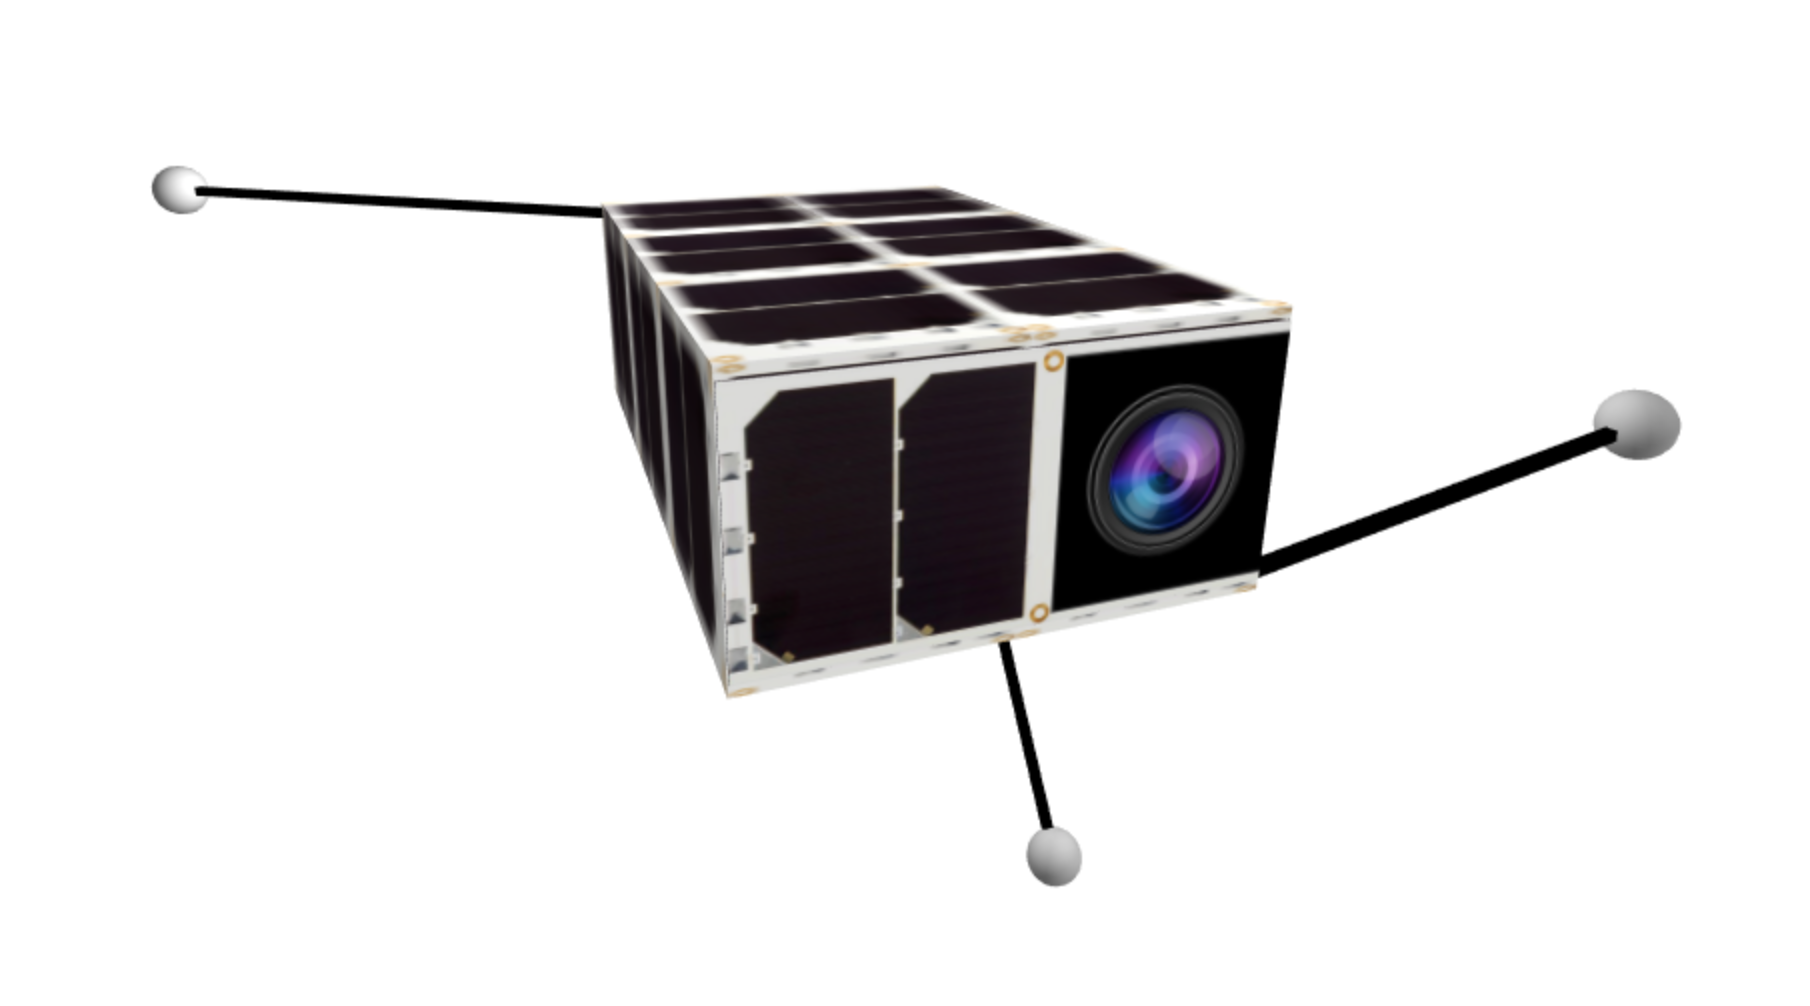
\includegraphics[width=12cm]{Figures/view1.png}
    \caption{Proposed architecture for a 6U CubeSat space telescope. Each boom has a single degree-of-freedom in linearly independent axes, enabling three-axis attitude control. Magnetorquers are used to desaturate the angular momentum of the booms and keep them within their operating limits.}
    \label{fig:meshcat_shot}
\end{figure}

In this paper, a novel actuation strategy for fine-pointing nanosatellites is explored by abandoning high-frequency rotor-based actuators in favor of low-frequency deployable booms, as shown in Figure \ref{fig:meshcat_shot}. By taking advantage of the squared relationship between boom length and the inertia of the boom, tip-mounted masses provide the control authority required for attitude control without having to accelerate or decelerate the booms too aggressively. A nanosatellite would deploy three booms about linearly independent axes and rotate them \textit{slowly} to reject the \textit{slowly} varying disturbance torques. By better matching the actuators' speed to the frequency content of the disturbances, these booms are able to eliminate jitter and enable high-accuracy body pointing of the nanosatellite. By improving body pointing, payloads are no longer restricted to those that can accommodate second-stage correction, and existing payloads can be simplified. 

For nanosatellites in low-Earth orbit, disturbance torques come in the form of drag, solar radiation pressure, magnetic, and gravity-gradient torques. All of these disturbances vary slowly throughout an orbit and can be predicted or estimated with high accuracy.  With knowledge of the incoming disturbance torques, the nanosatellite can formulate a motion plan that accounts for disturbances and keeps the deployable booms from hitting their hard stops by using the onboard magnetorquers to offload angular momentum through interactions with the Earth's magnetic field \cite{gatherer2019,markley2014}. Since nominal operations have the nanosatellites inertially pointing during payload operations, linearized attitude dynamics are sufficiently accurate for planning purposes. This allows for a convex formulation of the motion-planning problem, guaranteeing a globally optimal solution in polynomial time \cite{boyd2004}. 

Our primary contributions in this paper include:
%\vspace{-1em}
\begin{enumerate}
\item The introduction of a novel attitude-actuation strategy for fine-pointing nanosatellites.
\vspace{+2mm}
%\item A frequency analysis of the environmental disturbance torques present on a satellite in low-Earth orbit. \todo{this is from our other paper technically}
\vspace{+2mm}
\item The application of convex optimization to motion planning for nanosatellites with actuated booms.
\vspace{+2mm}
\item An estimator and controller architecture for handling boom control during payload operations.
\end{enumerate}
%\vspace{-1em}

In the remainder of this paper, we first provide details on the simulation environment used for this research in Section~\ref{sec:wigglesat:simenv}. Next, the deployable-boom actuation strategy is discussed in Section \ref{sec:wigglesat:actuation}, and a convex motion planner is developed in Section \ref{sec:wigglesat:planner} to reason about the actuator's constraints.  A lower-level estimation and control architecture is then detailed in Section \ref{sec:wigglesat:control}. Finally, numerical experiments are presented in Section \ref{sec:wigglesat:experiments} to validate the proposed ideas, and results are summarized in Section \ref{sec:wigglesat:conclusion}.

\section{Spacecraft Dynamics Model}
\label{sec:wigglesat:simenv}
This section describes the model used to analyze and simulate the dynamics of a nanosatellite space telescope in low-Earth orbit. Since the spacecraft has no propulsion onboard, the orbital and attitude dynamics are decoupled and can be modeled separately. The open-source Julia package \textit{SatelliteDynamics.jl} is used for orbital simulation, taking into account high order gravity, atmospheric drag, solar radiation pressure, and third-body accelerations. For the attitude dynamics, a rigid-body simulation is used that includes the disturbance torques present in low-Earth orbit. 

We denote the Earth-Centered Inertial frame (ECI) as $\mathbb{E}$, and the spacecraft body frame as $\mathbb{B}$. Relating these two frames is ${}^{\mathbb{B}} Q {}^{\mathbb{E}}$, the rotation matrix that takes vectors expressed in $\mathbb{E}$ and resolves them in frame $\mathbb{B}$.
\subsubsection{Gravity-Gradient Torque}
Gravity varies inversely with the square of the distance from the central body. Because of this, parts of the spacecraft that are farther away from the center of the central body experience a smaller gravitational force than the parts that are closer. The resulting non-uniform gravitational force acting on the spacecraft causes a torque. This torque can be neatly expressed in terms of the spacecraft's attitude, orbital position, and the inertia \cite{markley2014,wertz1978}. First, the normalized position vector is computed in the body frame:
\begin{align}
    \hat{m} &= \frac{{}^{\mathbb{B}} Q {}^{\mathbb{E}} r_{\mathbb{E}}}{\|r_{\mathbb{E}}\|},
\end{align}
then, the gravity-gradient torque can be calculated, 
\begin{align}
    \tau_{gg} &= \frac{3 \mu}{\|r\|^3}(\hat{m} \times J\hat{m}),
\end{align}
where $\mu$ is the standard gravitational parameter for Earth. This calculation only takes into consideration the spherical gravitational term, since the gravity gradient torque from higher-order gravity terms is of negligible magnitude.  For inertially pointing spacecraft in pure Keplerian motion, the resulting gravity gradient torque is periodic with the orbit.

\subsubsection{Atmospheric Drag Torque}
To describe the atmospheric drag torque, the relative velocity of the spacecraft with respect to the atmosphere is calculated with the following:
\begin{align}
    v_{rel} = {}^{\mathbb{B}} Q {}^{\mathbb{E}} ( v_{eci} - \omega_{Earth} \times r_{\mathbb{E}} ).
\end{align}
A normalized version of this vector will be represented as $\hat{v}_{rel} = v_{rel}/\|v_{rel}\|$.
The spacecraft in this experiment has been parameterized as a box with 6 orthogonal faces. This geometry is described with normal vectors $\hat{n}_i$ for each face, position vectors from the center of mass of the spacecraft to the center of pressure of each face $r_i$, and the area of each face $S_i$. Only the faces in the direction of the relative velocity vector are affected, and the force is proportional to the cosine of the angle between the normal face vector and the relative velocity vector. This can also be represented as the dot product between two normalized vectors:
\begin{align}
w_i &= \text{max}(0,v^T [^{\mathbb{E}}Q^{\mathbb{B}} \, \hat{n}_i]).
\end{align}
The force on each face is then calculated with the atmospheric density $\rho$ and the coefficient of drag $C_d$, 
\begin{align}
    F_{aero,i} &= -\frac{1}{2}\rho\, C_d \|v_{rel}\| v_{rel}S_i w_i.
\end{align}
The torque acting on the nanosatelite is then the sum of the moments caused by these forces:
\begin{align}
     \tau_{aero} &=  \sum_{i = 1}^6 r_i \times  F_{aero,i}.
\end{align}
\subsubsection{Solar Radiation Pressure Torque}
Similar to the aerodynamic drag torque, the radiation from the sun carries momentum, and can impart a force on the spacecraft. First, the position vector from the spacecraft to the sun is calculated as:
\begin{align}
    {}^{\mathbb{B}}r{}^{sun} &= {}^{\mathbb{E}}r{}^{sun} - {}^{\mathbb{E}}r{}^{\mathbb{B}},
\end{align}
after which it is expressed in the body frame and normalized:
\begin{align}
     \hat{s} &= \frac{ {}^{\mathbb{B}} Q {}^{\mathbb{E}} \,\,{}^{\mathbb{B}}r{}^{sun}}{\| {}^{\mathbb{B}}r{}^{sun}\|}.
\end{align}
% \begin{align}
%     {}^{B}r{}^{sun} &= {}^{E}r{}^{sun} - {}^{E}r{}^{B} \\ \hat{s} &= \frac{ {}^B Q {}^N, {}^{B}r{}^{sun}}{\| {}^{B}r{}^{sun}\|}.
% \end{align}
Based on the spectral and diffuse reflection coefficients, $R_{spec}$ and $R_{diff}$ respectively, the optical properties of the spacecraft material with respect to solar radiation pressure can be calculated. The combined effects of reflection, diffusion, and absorption are captured in our variable $q_i$, 
\begin{align}
    q_i &=  2\big[ \frac{1}{3}R_{diff} + R_{spec} \hat{s}^T \hat{n}_i\big] \hat{n}_i + (1 - R_{spec})\hat{s}. 
\end{align}
The force caused by radiation pressure on each face is then, 
\begin{align}
    F_{srp,i} &= -P_{sun} S_i q_i \cdot \text{max}(0,\hat{s}^T [^{\mathbb{E}}Q^{\mathbb{B}} \, n_i]),
\end{align}
and the final torque is the sum of the moments caused by the force on each face:
\begin{align}
    \tau_{srp} &=  \sum_{i = 1}^6 r_i \times  F_{srp,i}.
\end{align}
\subsubsection{Magnetic Torques}
We use the International Geomagnetic Reference Field (IGRF) \cite{thebault2015} to model the Earth's magnetic field. The IGRF models the scalar potential of the magnetic field with a spherical harmonic expansion and calculates the magnetic field vector as the negative gradient of this potential with respect to the position.  This potential is described by a set of time-varying coefficients that account for decades of empirical data and can predict the Earth's magnetic field up to 5 years in the future. This resulting magnetic field vector is a function of position and time, and for spacecraft with no propulsion, can be computed online to predict future magnetometer measurements. The spacecraft can then use the onboard magnetorquers to interact with the Earth's magnetic field in the following way:
\begin{align}
    \tau_{mag} = m \times b_{\mathbb{B}},
\end{align}
where $b_{\mathbb{B}}$ is the magnetic field vector expressed in the spacecraft body frame, and $m$ is the spacecraft's magnetic moment in the body frame. The total disturbance torque on the nanosatellite is the sum of the aforementioned torques:
\begin{align}
    \tau = \tau_{gg} + \tau_{aero} + \tau_{srp} + \tau_{mag}.
\end{align}
\section{Actuation Strategy}
\label{sec:wigglesat:actuation}
To justify the introduction of a novel actuation strategy, the nature of the disturbance torques was analyzed.  A 1000-trial Monte-Carlo simulation of the orbital and attitude dynamics was performed and disturbance torques were collected. The orbits in the simulations were at an altitude of 550 km with inclinations between 0$^\circ$ and 90$^\circ$, eccentricities between 0 and 0.00002, and epochs between 2014 and 2017. These dispersions served to capture the full range of potential disturbance torques, as well as accurately sample the time-varying atmospheric density.  A discrete Fourier transform of the disturbance torque data was taken, and the magnitudes of the terms in the Fourier series were used to plot its power-spectral density in Figure \ref{fig:disturbances}. 
\begin{figure}%[H]
    \centering
    % \setlength{\figureheight}{3.0in}
    % \setlength{\figurewidth}{5.0in}
    % % This file was created by matlab2tikz.
%
%The latest updates can be retrieved from
%  http://www.mathworks.com/matlabcentral/fileexchange/22022-matlab2tikz-matlab2tikz
%where you can also make suggestions and rate matlab2tikz.
%
\begin{tikzpicture}

\begin{axis}[%
width=4in,
height=2.0in,
at={(0,0)},
scale only axis,
xmode=log,
xmin=0.0001,
xmax=1000,
xminorticks=true,
xlabel style={font=\color{white!15!black}},
xlabel={Frequency (Hz)},
ymode=log,
ymin=0.01,
ymax=100,
yminorticks=true,
ylabel style={font=\color{white!15!black}},
ylabel={$\text{RMS Torque}\mu N \cdot m/\sqrt{Hz}$},
axis background/.style={fill=white},
axis x line*=bottom,
axis y line*=left,
% legend style={legend cell align=left, align=left, draw=white!15!black}
% ]
legend style={at={(0.5,-0.3)}, anchor=north, legend cell align=left, align=left, draw=white!15!black}
]
\addplot [color=black, forget plot]
  table[row sep=crcr]{%
0	0\\
1e-06	0\\
2e-06	0\\
3e-06	0\\
4e-06	0\\
5e-06	0\\
6e-06	0\\
7e-06	0\\
8e-06	0\\
9e-06	0\\
1e-05	0\\
1.1e-05	0\\
1.2e-05	0\\
1.3e-05	0\\
1.4e-05	0\\
1.5e-05	0\\
1.6e-05	0\\
1.7e-05	0\\
1.8e-05	0\\
1.9e-05	0\\
2e-05	0\\
2.1e-05	0\\
2.2e-05	0\\
2.3e-05	0\\
2.4e-05	0\\
2.5e-05	0\\
2.6e-05	0\\
2.7e-05	0\\
2.8e-05	0\\
2.9e-05	0\\
3e-05	0\\
3.1e-05	0\\
3.2e-05	0\\
3.3e-05	0\\
3.4e-05	0\\
3.5e-05	0\\
3.6e-05	0\\
3.7e-05	0\\
3.8e-05	0\\
3.9e-05	0\\
4e-05	0\\
4.1e-05	0\\
4.2e-05	0\\
4.3e-05	0\\
4.4e-05	0\\
4.5e-05	0\\
4.6e-05	0\\
4.7e-05	0\\
4.8e-05	0\\
4.9e-05	0\\
5e-05	0\\
5.1e-05	0\\
5.2e-05	0\\
5.3e-05	0\\
5.4e-05	0\\
5.5e-05	0\\
5.6e-05	0\\
5.7e-05	0\\
5.8e-05	0\\
5.9e-05	0\\
6e-05	0\\
6.1e-05	0\\
6.2e-05	0\\
6.3e-05	0\\
6.4e-05	0\\
6.5e-05	0\\
6.6e-05	0\\
6.7e-05	0\\
6.8e-05	0\\
6.9e-05	0\\
7e-05	0\\
7.1e-05	0\\
7.2e-05	0\\
7.3e-05	0\\
7.4e-05	0\\
7.5e-05	0\\
7.6e-05	0\\
7.7e-05	0\\
7.8e-05	0\\
7.9e-05	0\\
8e-05	0.247\\
8.1e-05	0.247\\
8.2e-05	0.247\\
8.3e-05	0.248\\
8.4e-05	0.248\\
8.5e-05	0.249\\
8.6e-05	0.249\\
8.7e-05	0.249\\
8.8e-05	0.25\\
8.9e-05	0.251\\
9e-05	0.252\\
9.1e-05	0.253\\
9.2e-05	0.253\\
9.3e-05	0.254\\
9.4e-05	0.255\\
9.5e-05	0.256\\
9.6e-05	0.256\\
9.7e-05	0.257\\
9.8e-05	0.258\\
9.9e-05	0.259\\
0.0001	0.26\\
0.000101	0.26\\
0.000102	0.261\\
0.000103	0.262\\
0.000104	0.263\\
0.000105	0.264\\
0.000106	0.265\\
0.000107	0.266\\
0.000108	0.268\\
0.000109	0.269\\
0.00011	0.27\\
0.000111	0.272\\
0.000112	0.273\\
0.000113	0.274\\
0.000114	0.275\\
0.000115	0.277\\
0.000116	0.278\\
0.000117	0.279\\
0.000118	0.281\\
0.000119	0.282\\
0.00012	0.283\\
0.000121	0.285\\
0.000122	0.286\\
0.000123	0.288\\
0.000124	0.29\\
0.000125	0.293\\
0.000126	0.295\\
0.000127	0.297\\
0.000128	0.3\\
0.000129	0.302\\
0.00013	0.304\\
0.000131	0.307\\
0.000132	0.309\\
0.000133	0.311\\
0.000134	0.313\\
0.000135	0.316\\
0.000136	0.318\\
0.000137	0.32\\
0.000138	0.323\\
0.000139	0.325\\
0.00014	0.329\\
0.000141	0.335\\
0.000142	0.341\\
0.000143	0.347\\
0.000144	0.353\\
0.000145	0.359\\
0.000146	0.365\\
0.000147	0.371\\
0.000148	0.377\\
0.000149	0.383\\
0.00015	0.389\\
0.000151	0.395\\
0.000152	0.401\\
0.000153	0.407\\
0.000154	0.413\\
0.000155	0.419\\
0.000156	0.425\\
0.000157	0.524\\
0.000158	1.25\\
0.000159	1.98\\
0.00016	2.72\\
0.000161	3.45\\
0.000162	4.19\\
0.000163	4.92\\
0.000164	5.65\\
0.000165	6.39\\
0.000166	7.12\\
0.000167	7.86\\
0.000168	8.59\\
0.000169	9.33\\
0.00017	10.1\\
0.000171	10.8\\
0.000172	11.5\\
0.000173	12.3\\
0.000174	13\\
0.000175	12.6\\
0.000176	11.9\\
0.000177	11.2\\
0.000178	10.4\\
0.000179	9.7\\
0.00018	8.97\\
0.000181	8.23\\
0.000182	7.5\\
0.000183	6.77\\
0.000184	6.04\\
0.000185	5.31\\
0.000186	4.57\\
0.000187	3.84\\
0.000188	3.11\\
0.000189	2.38\\
0.00019	1.65\\
0.000191	0.915\\
0.000192	0.424\\
0.000193	0.418\\
0.000194	0.413\\
0.000195	0.408\\
0.000196	0.402\\
0.000197	0.397\\
0.000198	0.392\\
0.000199	0.386\\
0.0002	0.381\\
0.000201	0.376\\
0.000202	0.371\\
0.000203	0.365\\
0.000204	0.36\\
0.000205	0.355\\
0.000206	0.349\\
0.000207	0.344\\
0.000208	0.339\\
0.000209	0.333\\
0.00021	0.333\\
0.000211	0.333\\
0.000212	0.333\\
0.000213	0.333\\
0.000214	0.333\\
0.000215	0.333\\
0.000216	0.333\\
0.000217	0.333\\
0.000218	0.334\\
0.000219	0.334\\
0.00022	0.335\\
0.000221	0.336\\
0.000222	0.337\\
0.000223	0.337\\
0.000224	0.338\\
0.000225	0.339\\
0.000226	0.34\\
0.000227	0.341\\
0.000228	0.343\\
0.000229	0.345\\
0.00023	0.347\\
0.000231	0.349\\
0.000232	0.352\\
0.000233	0.354\\
0.000234	0.356\\
0.000235	0.358\\
0.000236	0.36\\
0.000237	0.362\\
0.000238	0.364\\
0.000239	0.366\\
0.00024	0.369\\
0.000241	0.371\\
0.000242	0.373\\
0.000243	0.375\\
0.000244	0.377\\
0.000245	0.381\\
0.000246	0.384\\
0.000247	0.388\\
0.000248	0.391\\
0.000249	0.395\\
0.00025	0.398\\
0.000251	0.401\\
0.000252	0.405\\
0.000253	0.408\\
0.000254	0.412\\
0.000255	0.415\\
0.000256	0.419\\
0.000257	0.423\\
0.000258	0.427\\
0.000259	0.432\\
0.00026	0.436\\
0.000261	0.441\\
0.000262	0.447\\
0.000263	0.454\\
0.000264	0.46\\
0.000265	0.467\\
0.000266	0.473\\
0.000267	0.48\\
0.000268	0.486\\
0.000269	0.493\\
0.00027	0.5\\
0.000271	0.506\\
0.000272	0.513\\
0.000273	0.519\\
0.000274	0.526\\
0.000275	0.533\\
0.000276	0.539\\
0.000277	0.546\\
0.000278	0.552\\
0.000279	0.56\\
0.00028	0.57\\
0.000281	0.581\\
0.000282	0.592\\
0.000283	0.602\\
0.000284	0.613\\
0.000285	0.624\\
0.000286	0.634\\
0.000287	0.645\\
0.000288	0.656\\
0.000289	0.667\\
0.00029	0.677\\
0.000291	0.688\\
0.000292	0.699\\
0.000293	0.709\\
0.000294	0.72\\
0.000295	0.731\\
0.000296	0.741\\
0.000297	0.76\\
0.000298	0.781\\
0.000299	0.802\\
0.0003	0.823\\
0.000301	0.844\\
0.000302	0.865\\
0.000303	0.886\\
0.000304	0.907\\
0.000305	0.928\\
0.000306	0.949\\
0.000307	0.97\\
0.000308	0.991\\
0.000309	1.01\\
0.00031	1.03\\
0.000311	1.05\\
0.000312	1.07\\
0.000313	1.1\\
0.000314	1.13\\
0.000315	1.19\\
0.000316	1.25\\
0.000317	1.31\\
0.000318	1.37\\
0.000319	1.43\\
0.00032	1.5\\
0.000321	1.56\\
0.000322	1.62\\
0.000323	1.68\\
0.000324	1.74\\
0.000325	1.8\\
0.000326	1.86\\
0.000327	1.92\\
0.000328	1.98\\
0.000329	2.04\\
0.00033	2.1\\
0.000331	2.16\\
0.000332	4.7\\
0.000333	7.41\\
0.000334	10.1\\
0.000335	12.8\\
0.000336	15.6\\
0.000337	18.3\\
0.000338	21\\
0.000339	23.7\\
0.00034	26.4\\
0.000341	29.1\\
0.000342	31.9\\
0.000343	34.6\\
0.000344	37.3\\
0.000345	40\\
0.000346	42.7\\
0.000347	45.4\\
0.000348	48.1\\
0.000349	48.1\\
0.00035	45.4\\
0.000351	42.7\\
0.000352	40\\
0.000353	37.3\\
0.000354	34.6\\
0.000355	31.9\\
0.000356	29.2\\
0.000357	26.5\\
0.000358	23.8\\
0.000359	21.1\\
0.00036	18.4\\
0.000361	15.7\\
0.000362	13\\
0.000363	10.3\\
0.000364	7.57\\
0.000365	4.86\\
0.000366	2.38\\
0.000367	2.31\\
0.000368	2.24\\
0.000369	2.17\\
0.00037	2.1\\
0.000371	2.03\\
0.000372	1.96\\
0.000373	1.89\\
0.000374	1.82\\
0.000375	1.75\\
0.000376	1.68\\
0.000377	1.61\\
0.000378	1.54\\
0.000379	1.47\\
0.00038	1.4\\
0.000381	1.33\\
0.000382	1.26\\
0.000383	1.19\\
0.000384	1.15\\
0.000385	1.13\\
0.000386	1.1\\
0.000387	1.08\\
0.000388	1.06\\
0.000389	1.04\\
0.00039	1.01\\
0.000391	0.99\\
0.000392	0.967\\
0.000393	0.945\\
0.000394	0.922\\
0.000395	0.9\\
0.000396	0.877\\
0.000397	0.855\\
0.000398	0.832\\
0.000399	0.81\\
0.0004	0.787\\
0.000401	0.767\\
0.000402	0.756\\
0.000403	0.745\\
0.000404	0.734\\
0.000405	0.723\\
0.000406	0.712\\
0.000407	0.701\\
0.000408	0.69\\
0.000409	0.679\\
0.00041	0.668\\
0.000411	0.657\\
0.000412	0.646\\
0.000413	0.635\\
0.000414	0.624\\
0.000415	0.613\\
0.000416	0.602\\
0.000417	0.591\\
0.000418	0.58\\
0.000419	0.572\\
0.00042	0.566\\
0.000421	0.559\\
0.000422	0.553\\
0.000423	0.546\\
0.000424	0.54\\
0.000425	0.533\\
0.000426	0.527\\
0.000427	0.52\\
0.000428	0.514\\
0.000429	0.507\\
0.00043	0.501\\
0.000431	0.494\\
0.000432	0.488\\
0.000433	0.481\\
0.000434	0.474\\
0.000435	0.468\\
0.000436	0.462\\
0.000437	0.458\\
0.000438	0.454\\
0.000439	0.45\\
0.00044	0.445\\
0.000441	0.441\\
0.000442	0.437\\
0.000443	0.433\\
0.000444	0.429\\
0.000445	0.424\\
0.000446	0.42\\
0.000447	0.416\\
0.000448	0.412\\
0.000449	0.408\\
0.00045	0.403\\
0.000451	0.399\\
0.000452	0.395\\
0.000453	0.391\\
0.000454	0.388\\
0.000455	0.385\\
0.000456	0.382\\
0.000457	0.379\\
0.000458	0.377\\
0.000459	0.374\\
0.00046	0.371\\
0.000461	0.368\\
0.000462	0.365\\
0.000463	0.363\\
0.000464	0.36\\
0.000465	0.357\\
0.000466	0.354\\
0.000467	0.351\\
0.000468	0.349\\
0.000469	0.346\\
0.00047	0.343\\
0.000471	0.341\\
0.000472	0.339\\
0.000473	0.337\\
0.000474	0.336\\
0.000475	0.334\\
0.000476	0.332\\
0.000477	0.331\\
0.000478	0.329\\
0.000479	0.329\\
0.00048	0.329\\
0.000481	0.328\\
0.000482	0.328\\
0.000483	0.328\\
0.000484	0.328\\
0.000485	0.328\\
0.000486	0.327\\
0.000487	0.327\\
0.000488	0.327\\
0.000489	0.331\\
0.00049	0.334\\
0.000491	0.338\\
0.000492	0.341\\
0.000493	0.344\\
0.000494	0.348\\
0.000495	0.351\\
0.000496	0.355\\
0.000497	0.358\\
0.000498	0.361\\
0.000499	0.365\\
0.0005	0.368\\
0.000501	0.372\\
0.000502	0.375\\
0.000503	0.378\\
0.000504	0.382\\
0.000505	0.385\\
0.000506	0.501\\
0.000507	0.701\\
0.000508	0.902\\
0.000509	1.1\\
0.00051	1.3\\
0.000511	1.5\\
0.000512	1.7\\
0.000513	1.9\\
0.000514	2.1\\
0.000515	2.3\\
0.000516	2.5\\
0.000517	2.7\\
0.000518	2.91\\
0.000519	3.11\\
0.00052	3.31\\
0.000521	3.51\\
0.000522	3.71\\
0.000523	3.8\\
0.000524	3.6\\
0.000525	3.4\\
0.000526	3.2\\
0.000527	2.99\\
0.000528	2.79\\
0.000529	2.59\\
0.00053	2.39\\
0.000531	2.19\\
0.000532	1.99\\
0.000533	1.78\\
0.000534	1.58\\
0.000535	1.38\\
0.000536	1.18\\
0.000537	0.976\\
0.000538	0.774\\
0.000539	0.577\\
0.00054	0.389\\
0.000541	0.353\\
0.000542	0.346\\
0.000543	0.338\\
0.000544	0.332\\
0.000545	0.326\\
0.000546	0.321\\
0.000547	0.315\\
0.000548	0.309\\
0.000549	0.304\\
0.00055	0.298\\
0.000551	0.293\\
0.000552	0.287\\
0.000553	0.281\\
0.000554	0.276\\
0.000555	0.27\\
0.000556	0.264\\
0.000557	0.259\\
0.000558	0.255\\
0.000559	0.253\\
0.00056	0.25\\
0.000561	0.248\\
0.000562	0.246\\
0.000563	0.244\\
0.000564	0.242\\
0.000565	0.24\\
0.000566	0.238\\
0.000567	0.235\\
0.000568	0.233\\
0.000569	0.231\\
0.00057	0.229\\
0.000571	0.227\\
0.000572	0.225\\
0.000573	0.223\\
0.000574	0.22\\
0.000575	0.218\\
0.000576	0.217\\
0.000577	0.216\\
0.000578	0.215\\
0.000579	0.213\\
0.00058	0.212\\
0.000581	0.211\\
0.000582	0.21\\
0.000583	0.208\\
0.000584	0.207\\
0.000585	0.206\\
0.000586	0.205\\
0.000587	0.204\\
0.000588	0.203\\
0.000589	0.202\\
0.00059	0.201\\
0.000591	0.2\\
0.000592	0.198\\
0.000593	0.198\\
0.000594	0.197\\
0.000595	0.196\\
0.000596	0.195\\
0.000597	0.194\\
0.000598	0.194\\
0.000599	0.193\\
0.0006	0.192\\
0.000601	0.191\\
0.000602	0.191\\
0.000603	0.19\\
0.000604	0.189\\
0.000605	0.188\\
0.000606	0.188\\
0.000607	0.187\\
0.000608	0.186\\
0.000609	0.185\\
0.00061	0.185\\
0.000611	0.184\\
0.000612	0.183\\
0.000613	0.183\\
0.000614	0.182\\
0.000615	0.182\\
0.000616	0.181\\
0.000617	0.181\\
0.000618	0.18\\
0.000619	0.18\\
0.00062	0.179\\
0.000621	0.179\\
0.000622	0.178\\
0.000623	0.177\\
0.000624	0.177\\
0.000625	0.176\\
0.000626	0.176\\
0.000627	0.175\\
0.000628	0.175\\
0.000629	0.174\\
0.00063	0.174\\
0.000631	0.174\\
0.000632	0.173\\
0.000633	0.173\\
0.000634	0.173\\
0.000635	0.172\\
0.000636	0.172\\
0.000637	0.172\\
0.000638	0.171\\
0.000639	0.171\\
0.00064	0.171\\
0.000641	0.17\\
0.000642	0.17\\
0.000643	0.17\\
0.000644	0.169\\
0.000645	0.169\\
0.000646	0.169\\
0.000647	0.169\\
0.000648	0.169\\
0.000649	0.169\\
0.00065	0.169\\
0.000651	0.169\\
0.000652	0.169\\
0.000653	0.17\\
0.000654	0.17\\
0.000655	0.17\\
0.000656	0.17\\
0.000657	0.17\\
0.000658	0.17\\
0.000659	0.171\\
0.00066	0.171\\
0.000661	0.171\\
0.000662	0.171\\
0.000663	0.172\\
0.000664	0.174\\
0.000665	0.175\\
0.000666	0.177\\
0.000667	0.178\\
0.000668	0.179\\
0.000669	0.181\\
0.00067	0.182\\
0.000671	0.184\\
0.000672	0.185\\
0.000673	0.187\\
0.000674	0.188\\
0.000675	0.189\\
0.000676	0.191\\
0.000677	0.192\\
0.000678	0.194\\
0.000679	0.195\\
0.00068	0.216\\
0.000681	0.261\\
0.000682	0.307\\
0.000683	0.361\\
0.000684	0.422\\
0.000685	0.482\\
0.000686	0.542\\
0.000687	0.603\\
0.000688	0.667\\
0.000689	0.736\\
0.00069	0.805\\
0.000691	0.875\\
0.000692	0.944\\
0.000693	1.01\\
0.000694	1.08\\
0.000695	1.15\\
0.000696	1.22\\
0.000697	1.29\\
0.000698	1.22\\
0.000699	1.15\\
0.0007	1.08\\
0.000701	1.01\\
0.000702	0.944\\
0.000703	0.875\\
0.000704	0.806\\
0.000705	0.743\\
0.000706	0.685\\
0.000707	0.627\\
0.000708	0.57\\
0.000709	0.512\\
0.00071	0.454\\
0.000711	0.396\\
0.000712	0.339\\
0.000713	0.281\\
0.000714	0.223\\
0.000715	0.198\\
0.000716	0.194\\
0.000717	0.191\\
0.000718	0.188\\
0.000719	0.185\\
0.00072	0.182\\
0.000721	0.178\\
0.000722	0.175\\
0.000723	0.172\\
0.000724	0.169\\
0.000725	0.166\\
0.000726	0.162\\
0.000727	0.159\\
0.000728	0.156\\
0.000729	0.153\\
0.00073	0.15\\
0.000731	0.146\\
0.000732	0.144\\
0.000733	0.143\\
0.000734	0.142\\
0.000735	0.141\\
0.000736	0.14\\
0.000737	0.139\\
0.000738	0.138\\
0.000739	0.138\\
0.00074	0.137\\
0.000741	0.136\\
0.000742	0.135\\
0.000743	0.134\\
0.000744	0.133\\
0.000745	0.132\\
0.000746	0.131\\
0.000747	0.131\\
0.000748	0.13\\
0.000749	0.129\\
0.00075	0.128\\
0.000751	0.128\\
0.000752	0.127\\
0.000753	0.127\\
0.000754	0.126\\
0.000755	0.126\\
0.000756	0.125\\
0.000757	0.125\\
0.000758	0.124\\
0.000759	0.124\\
0.00076	0.123\\
0.000761	0.123\\
0.000762	0.122\\
0.000763	0.122\\
0.000764	0.121\\
0.000765	0.121\\
0.000766	0.12\\
0.000767	0.12\\
0.000768	0.12\\
0.000769	0.119\\
0.00077	0.119\\
0.000771	0.119\\
0.000772	0.119\\
0.000773	0.118\\
0.000774	0.118\\
0.000775	0.118\\
0.000776	0.117\\
0.000777	0.117\\
0.000778	0.117\\
0.000779	0.116\\
0.00078	0.116\\
0.000781	0.116\\
0.000782	0.116\\
0.000783	0.115\\
0.000784	0.115\\
0.000785	0.115\\
0.000786	0.115\\
0.000787	0.114\\
0.000788	0.114\\
0.000789	0.114\\
0.00079	0.114\\
0.000791	0.113\\
0.000792	0.113\\
0.000793	0.113\\
0.000794	0.113\\
0.000795	0.113\\
0.000796	0.112\\
0.000797	0.112\\
0.000798	0.112\\
0.000799	0.112\\
0.0008	0.112\\
0.000801	0.111\\
0.000802	0.111\\
0.000803	0.111\\
0.000804	0.111\\
0.000805	0.111\\
0.000806	0.111\\
0.000807	0.112\\
0.000808	0.112\\
0.000809	0.112\\
0.00081	0.112\\
0.000811	0.113\\
0.000812	0.113\\
0.000813	0.113\\
0.000814	0.113\\
0.000815	0.113\\
0.000816	0.114\\
0.000817	0.114\\
0.000818	0.114\\
0.000819	0.114\\
0.00082	0.115\\
0.000821	0.115\\
0.000822	0.116\\
0.000823	0.116\\
0.000824	0.117\\
0.000825	0.118\\
0.000826	0.118\\
0.000827	0.119\\
0.000828	0.119\\
0.000829	0.12\\
0.00083	0.12\\
0.000831	0.121\\
0.000832	0.121\\
0.000833	0.122\\
0.000834	0.123\\
0.000835	0.123\\
0.000836	0.124\\
0.000837	0.125\\
0.000838	0.127\\
0.000839	0.129\\
0.00084	0.131\\
0.000841	0.133\\
0.000842	0.135\\
0.000843	0.137\\
0.000844	0.139\\
0.000845	0.141\\
0.000846	0.143\\
0.000847	0.145\\
0.000848	0.147\\
0.000849	0.149\\
0.00085	0.151\\
0.000851	0.153\\
0.000852	0.155\\
0.000853	0.157\\
0.000854	0.166\\
0.000855	0.203\\
0.000856	0.253\\
0.000857	0.307\\
0.000858	0.361\\
0.000859	0.415\\
0.00086	0.469\\
0.000861	0.523\\
0.000862	0.576\\
0.000863	0.63\\
0.000864	0.684\\
0.000865	0.738\\
0.000866	0.792\\
0.000867	0.846\\
0.000868	0.9\\
0.000869	0.954\\
0.00087	1.01\\
0.000871	1.06\\
0.000872	1.04\\
0.000873	0.985\\
0.000874	0.934\\
0.000875	0.884\\
0.000876	0.833\\
0.000877	0.782\\
0.000878	0.731\\
0.000879	0.681\\
0.00088	0.63\\
0.000881	0.579\\
0.000882	0.528\\
0.000883	0.478\\
0.000884	0.427\\
0.000885	0.376\\
0.000886	0.325\\
0.000887	0.275\\
0.000888	0.224\\
0.000889	0.189\\
0.00089	0.184\\
0.000891	0.179\\
0.000892	0.174\\
0.000893	0.17\\
0.000894	0.165\\
0.000895	0.16\\
0.000896	0.155\\
0.000897	0.15\\
0.000898	0.145\\
0.000899	0.14\\
0.0009	0.135\\
0.000901	0.131\\
0.000902	0.126\\
0.000903	0.121\\
0.000904	0.116\\
0.000905	0.111\\
0.000906	0.106\\
0.000907	0.105\\
0.000908	0.103\\
0.000909	0.102\\
0.00091	0.101\\
0.000911	0.1\\
0.000912	0.099\\
0.000913	0.0979\\
0.000914	0.0968\\
0.000915	0.0957\\
0.000916	0.0946\\
0.000917	0.0936\\
0.000918	0.0925\\
0.000919	0.0916\\
0.00092	0.0909\\
0.000921	0.0902\\
0.000922	0.0895\\
0.000923	0.0887\\
0.000924	0.0883\\
0.000925	0.0881\\
0.000926	0.0878\\
0.000927	0.0876\\
0.000928	0.0873\\
0.000929	0.087\\
0.00093	0.0868\\
0.000931	0.0865\\
0.000932	0.0862\\
0.000933	0.086\\
0.000934	0.0857\\
0.000935	0.0855\\
0.000936	0.0852\\
0.000937	0.0849\\
0.000938	0.0847\\
0.000939	0.0844\\
0.00094	0.0841\\
0.000941	0.0839\\
0.000942	0.0837\\
0.000943	0.0835\\
0.000944	0.0833\\
0.000945	0.0832\\
0.000946	0.083\\
0.000947	0.0828\\
0.000948	0.0826\\
0.000949	0.0824\\
0.00095	0.0823\\
0.000951	0.0821\\
0.000952	0.0819\\
0.000953	0.0817\\
0.000954	0.0815\\
0.000955	0.0814\\
0.000956	0.0812\\
0.000957	0.081\\
0.000958	0.0808\\
0.000959	0.0807\\
0.00096	0.0805\\
0.000961	0.0804\\
0.000962	0.0803\\
0.000963	0.0802\\
0.000964	0.0801\\
0.000965	0.0799\\
0.000966	0.0798\\
0.000967	0.0797\\
0.000968	0.0796\\
0.000969	0.0795\\
0.00097	0.0793\\
0.000971	0.0792\\
0.000972	0.0791\\
0.000973	0.079\\
0.000974	0.0789\\
0.000975	0.0787\\
0.000976	0.0786\\
0.000977	0.0786\\
0.000978	0.0785\\
0.000979	0.0785\\
0.00098	0.0784\\
0.000981	0.0783\\
0.000982	0.0783\\
0.000983	0.0782\\
0.000984	0.0782\\
0.000985	0.0781\\
0.000986	0.078\\
0.000987	0.078\\
0.000988	0.0779\\
0.000989	0.0779\\
0.00099	0.0778\\
0.000991	0.0777\\
0.000992	0.0777\\
0.000993	0.0776\\
0.000994	0.0776\\
0.000995	0.0776\\
0.000996	0.0776\\
0.000997	0.0776\\
0.000998	0.0776\\
0.000999	0.0776\\
0.001	0.0776\\
0.00105	0.477\\
0.0011	0.0628\\
0.00115	0.0596\\
0.0012	0.0862\\
0.00125	0.0736\\
0.0013	0.0558\\
0.00135	0.0531\\
0.0014	0.157\\
0.00145	0.0478\\
0.0015	0.0452\\
0.00155	0.0618\\
0.0016	0.0675\\
0.00165	0.0429\\
0.0017	0.0411\\
0.00175	0.117\\
0.0018	0.041\\
0.00185	0.0407\\
0.0019	0.0552\\
0.00195	0.0428\\
0.002	0.0325\\
0.00205	0.0323\\
0.0021	0.0906\\
0.00215	0.0351\\
0.0022	0.0294\\
0.00225	0.0439\\
0.0023	0.0429\\
0.00235	0.0354\\
0.0024	0.0332\\
0.00245	0.0534\\
0.0025	0.0297\\
0.00255	0.0303\\
0.0026	0.0457\\
0.00265	0.031\\
0.0027	0.0268\\
0.00275	0.0252\\
0.0028	0.0316\\
0.00285	0.0259\\
0.0029	0.0255\\
0.00295	0.038\\
0.003	0.0301\\
0.00305	0.0213\\
0.0031	0.0218\\
0.00315	0.048\\
0.0032	0.0251\\
0.00325	0.0224\\
0.0033	0.0325\\
0.00335	0.0215\\
0.0034	0.0208\\
0.00345	0.0229\\
0.0035	0.05\\
0.00355	0.0186\\
0.0036	0.0188\\
0.00365	0.0311\\
0.0037	0.0205\\
0.00375	0.0193\\
0.0038	0.0199\\
0.00385	0.0326\\
0.0039	0.0174\\
0.00395	0.0178\\
0.004	0.0349\\
0.00405	0.0204\\
0.0041	0.0175\\
0.00415	0.0176\\
0.0042	0.0211\\
0.00425	0.0164\\
0.0043	0.0163\\
0.00435	0.0299\\
0.0044	0.0182\\
0.00445	0.0156\\
0.0045	0.0176\\
0.00455	0.0339\\
0.0046	0.0157\\
0.00465	0.0146\\
0.0047	0.028\\
0.00475	0.0153\\
0.0048	0.0148\\
0.00485	0.0153\\
0.0049	0.037\\
0.00495	0.0138\\
0.005	0.0135\\
0.00505	0.0323\\
0.0051	0.0142\\
0.00515	0.0137\\
0.0052	0.0138\\
0.00525	0.0219\\
0.0053	0.0129\\
0.00535	0.013\\
0.0054	0.0314\\
0.00545	0.0136\\
0.0055	0.0123\\
0.00555	0.0124\\
0.0056	0.0164\\
0.00565	0.0127\\
0.0057	0.0128\\
0.00575	0.0358\\
0.0058	0.0123\\
0.00585	0.0118\\
0.0059	0.0132\\
0.00595	0.0267\\
0.006	0.0113\\
0.00605	0.0115\\
0.0061	0.0282\\
0.00615	0.0128\\
0.0062	0.0114\\
0.00625	0.0125\\
0.0063	0.0208\\
0.00635	0.0102\\
0.0064	0.0104\\
0.00645	0.0228\\
0.0065	0.0103\\
0.00655	0.0104\\
0.0066	0.011\\
0.00665	0.0148\\
0.0067	0.0101\\
0.00675	0.0106\\
0.0068	0.0219\\
0.00685	0.00994\\
0.0069	0.00937\\
0.00695	0.0105\\
0.007	0.0103\\
0.00705	0.00965\\
0.0071	0.00996\\
0.00715	0.019\\
0.0072	0.00945\\
0.00725	0.00926\\
0.0073	0.0124\\
0.00735	0.011\\
0.0074	0.0086\\
0.00745	0.00882\\
0.0075	0.016\\
0.00755	0.0088\\
0.0076	0.00902\\
0.00765	0.00989\\
0.0077	0.0114\\
0.00775	0.00828\\
0.0078	0.00863\\
0.00785	0.0154\\
0.0079	0.00868\\
0.00795	0.00889\\
0.008	0.0087\\
0.00805	0.00938\\
0.0081	0.00834\\
0.00815	0.00867\\
0.0082	0.0198\\
0.00825	0.00758\\
0.0083	0.00781\\
0.00835	0.00974\\
0.0084	0.00761\\
0.00845	0.00768\\
0.0085	0.00792\\
0.00855	0.0167\\
0.0086	0.00789\\
0.00865	0.00762\\
0.0087	0.00984\\
0.00875	0.0111\\
0.0088	0.0073\\
0.00885	0.0074\\
0.0089	0.0149\\
0.00895	0.00718\\
0.009	0.00726\\
0.00905	0.00963\\
0.0091	0.0132\\
0.00915	0.00694\\
0.0092	0.00706\\
0.00925	0.0168\\
0.0093	0.00895\\
0.00935	0.00851\\
0.0094	0.00779\\
0.00945	0.00817\\
0.0095	0.0079\\
0.00955	0.00868\\
0.0096	0.0193\\
0.00965	0.00715\\
0.0097	0.00697\\
0.00975	0.0113\\
0.0098	0.00688\\
0.00985	0.00664\\
0.0099	0.00688\\
0.00995	0.017\\
0.01	0.00629\\
0.01005	0.00651\\
0.0101	0.0105\\
0.01015	0.0129\\
0.0102	0.00707\\
0.01025	0.00621\\
0.0103	0.0149\\
0.01035	0.00785\\
0.0104	0.00669\\
0.01045	0.0126\\
0.0105	0.0105\\
0.01055	0.0062\\
0.0106	0.00662\\
0.01065	0.0131\\
0.0107	0.0069\\
0.01075	0.00677\\
0.0108	0.0133\\
0.01085	0.00716\\
0.0109	0.00661\\
0.01095	0.00769\\
0.011	0.0133\\
0.01105	0.00657\\
0.0111	0.00626\\
0.01115	0.0144\\
0.0112	0.00609\\
0.01125	0.00587\\
0.0113	0.00581\\
0.01135	0.00995\\
0.0114	0.00594\\
0.01145	0.00611\\
0.0115	0.0111\\
0.01155	0.0095\\
0.0116	0.00583\\
0.01165	0.00597\\
0.0117	0.00933\\
0.01175	0.00711\\
0.0118	0.00578\\
0.01185	0.0114\\
0.0119	0.00665\\
0.01195	0.00545\\
0.012	0.006\\
0.01205	0.00936\\
0.0121	0.00543\\
0.01215	0.00534\\
0.0122	0.00898\\
0.01225	0.00582\\
0.0123	0.00551\\
0.01235	0.00554\\
0.0124	0.0111\\
0.01245	0.00579\\
0.0125	0.00543\\
0.01255	0.00813\\
0.0126	0.0055\\
0.01265	0.00534\\
0.0127	0.00574\\
0.01275	0.00939\\
0.0128	0.00549\\
0.01285	0.00548\\
0.0129	0.00819\\
0.01295	0.00571\\
0.013	0.00503\\
0.01305	0.00535\\
0.0131	0.00794\\
0.01315	0.00526\\
0.0132	0.00525\\
0.01325	0.00701\\
0.0133	0.00498\\
0.01335	0.00501\\
0.0134	0.00516\\
0.01345	0.0108\\
0.0135	0.00487\\
0.01355	0.0053\\
0.0136	0.00746\\
0.01365	0.00513\\
0.0137	0.0051\\
0.01375	0.00533\\
0.0138	0.0139\\
0.01385	0.00474\\
0.0139	0.00478\\
0.01395	0.00649\\
0.014	0.00502\\
0.01405	0.0048\\
0.0141	0.00486\\
0.01415	0.00907\\
0.0142	0.00482\\
0.01425	0.00496\\
0.0143	0.00935\\
0.01435	0.00491\\
0.0144	0.00469\\
0.01445	0.00586\\
0.0145	0.00707\\
0.01455	0.00468\\
0.0146	0.00475\\
0.01465	0.00739\\
0.0147	0.00564\\
0.01475	0.00461\\
0.0148	0.0056\\
0.01485	0.00864\\
0.0149	0.0046\\
0.01495	0.0054\\
0.015	0.00772\\
0.01505	0.0045\\
0.0151	0.00475\\
0.01515	0.0062\\
0.0152	0.00873\\
0.01525	0.00428\\
0.0153	0.00447\\
0.01535	0.00744\\
0.0154	0.00428\\
0.01545	0.00425\\
0.0155	0.00447\\
0.01555	0.00645\\
0.0156	0.00432\\
0.01565	0.00448\\
0.0157	0.00822\\
0.01575	0.00456\\
0.0158	0.00413\\
0.01585	0.005\\
0.0159	0.00429\\
0.01595	0.00409\\
0.016	0.00422\\
0.01605	0.00618\\
0.0161	0.00458\\
0.01615	0.00416\\
0.0162	0.00465\\
0.01625	0.00521\\
0.0163	0.00429\\
0.01635	0.00403\\
0.0164	0.00586\\
0.01645	0.00392\\
0.0165	0.00455\\
0.01655	0.00556\\
0.0166	0.00454\\
0.01665	0.00386\\
0.0167	0.00411\\
0.01675	0.00631\\
0.0168	0.00371\\
0.01685	0.00384\\
0.0169	0.00403\\
0.01695	0.00451\\
0.017	0.00384\\
0.01705	0.00399\\
0.0171	0.00634\\
0.01715	0.00443\\
0.0172	0.00374\\
0.01725	0.00387\\
0.0173	0.00422\\
0.01735	0.004\\
0.0174	0.00381\\
0.01745	0.00444\\
0.0175	0.00364\\
0.01755	0.00375\\
0.0176	0.00409\\
0.01765	0.00476\\
0.0177	0.0036\\
0.01775	0.00362\\
0.0178	0.0042\\
0.01785	0.00359\\
0.0179	0.00376\\
0.01795	0.00395\\
0.018	0.00408\\
0.01805	0.00358\\
0.0181	0.00398\\
0.01815	0.00444\\
0.0182	0.00347\\
0.01825	0.00348\\
0.0183	0.00348\\
0.01835	0.00412\\
0.0184	0.00354\\
0.01845	0.00361\\
0.0185	0.00449\\
0.01855	0.00342\\
0.0186	0.00345\\
0.01865	0.00368\\
0.0187	0.00372\\
0.01875	0.00344\\
0.0188	0.00341\\
0.01885	0.00375\\
0.0189	0.00343\\
0.01895	0.00346\\
0.019	0.00374\\
0.01905	0.00361\\
0.0191	0.00332\\
0.01915	0.00335\\
0.0192	0.0034\\
0.01925	0.00333\\
0.0193	0.00334\\
0.01935	0.00338\\
0.0194	0.00366\\
0.01945	0.00334\\
0.0195	0.00338\\
0.01955	0.00373\\
0.0196	0.00333\\
0.01965	0.00328\\
0.0197	0.0033\\
0.01975	0.00333\\
0.0198	0.00328\\
0.01985	0.00328\\
0.0199	0.00377\\
0.01995	0.00323\\
};
% \addlegendentry{Maximum RMS}
% \addlegendentry{}

\addplot[area legend, draw=black, fill=blue, draw opacity=0, fill opacity=0.3]
table[row sep=crcr] {%
x	y\\
10	0.0001\\
1000	0.0001\\
1000	100000000\\
10	100000000\\
}--cycle;
\addlegendentry{Reaction Wheel Control/Jitter}

\addplot[area legend, pattern = crosshatch, pattern color = black]
table[row sep=crcr] {%
x	y\\
100	0.0001\\
1000	0.0001\\
1000	100000000\\
100	100000000\\
}--cycle;
\addlegendentry{Structural Modes}

\end{axis}
\end{tikzpicture}%
% % This file was created by matlab2tikz.

    \includegraphics[width=6in]{Figures/mc_frequencies_2.tikz}
    \caption{The frequency content of disturbance torques on a small satellite in low-Earth orbit. Disturbances are due to atmospheric drag, solar radiation pressure, and the gravity gradient. The frequency content of the disturbances is of significantly lower frequency than both standard reaction wheels and structural modes of the nanosatellites.}
    \label{fig:disturbances}
    % \vspace{-10pt}
\end{figure}

Figure \ref{fig:disturbances} displays a clear mismatch between the speed of the disturbances and the speed of the actuators currently used in space telescopes. Jitter from traditional reaction wheels and the structural modes of the spacecraft is 3-4 orders of magnitude faster than the disturbance torques. This mismatch strongly suggests that slower actuators could be used, and as a result, interactions between the actuators and structural modes could be avoided. 

The proposed architecture is displayed in Figure \ref{fig:meshcat_shot}, with three masses mounted to deployable booms that will be used for full three-axis attitude control. Each deployable boom has a single-degree-of-freedom actuator at the interface between the boom and the spacecraft that can rotate the boom and mass combination. By moving the booms, angular momentum is transferred from the body of the spacecraft to the masses, allowing for full actuation of the spacecraft's attitude.  This actuation strategy is significantly slower than reaction wheels, and will therefore avoid both high-frequency jitter as well as the excitement of the flexible modes of the spacecraft. 

Two potential boom-actuator configurations are described in Figures \ref{fig:stepper} and \ref{fig:voice}, with a stepper motor and a linear voice coil respectively. Both of these actuators are able to precisely move the boom, but will also impart constraints on the torque, velocity, and configurations of the boom. These constraints will be accounted for by the onboard motion planner to ensure full attitude actuation is maintained. The boom actuators themselves can also contribute unwanted dynamics, like cogging torques and stiction, into the dynamics of the boom. Care must be taken when designing and building these actuators to ensure that these contributions to the dynamics are well characterized and incorporated into the planner. 
\begin{figure}
    \centering
    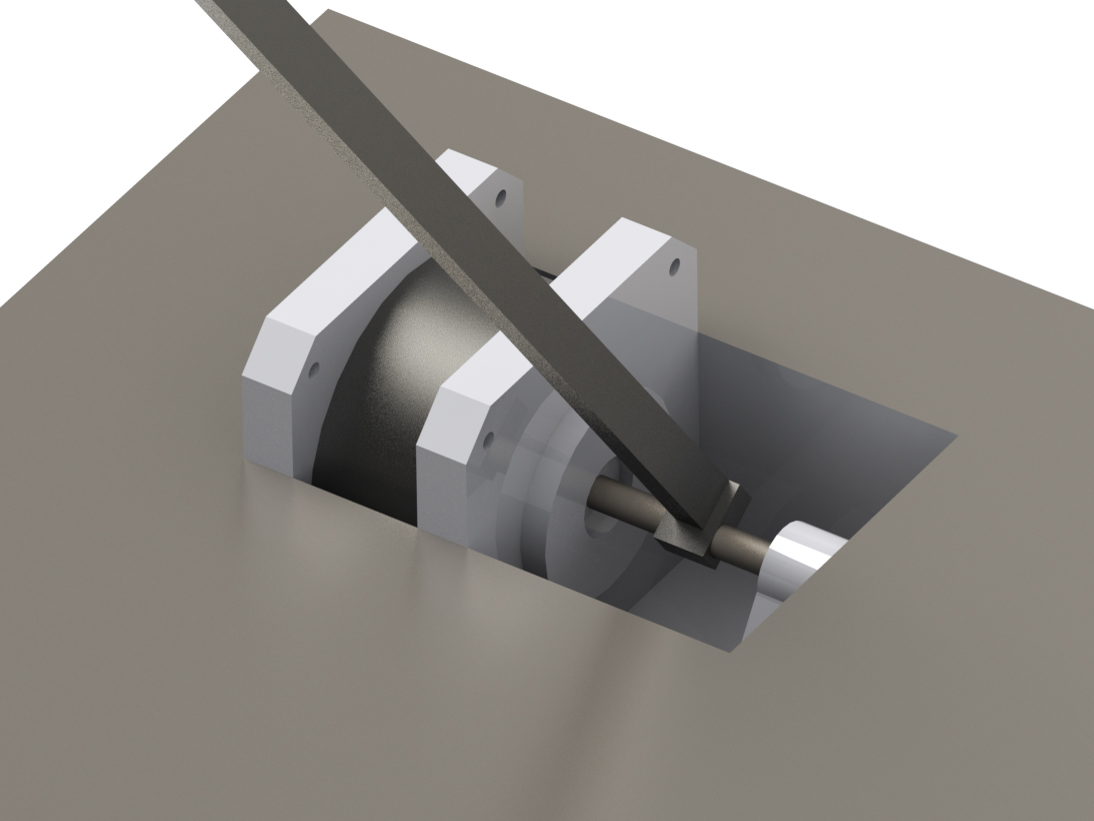
\includegraphics[width=.5\linewidth]{Figures/stepper_render.jpg}
    \caption{Boom actuation with a direct-drive micro-stepper motor. Torques commanded by the micro-stepper will accelerate and decelerate the boom, fully controlling the attitude of the nanosatellite.}
    \label{fig:stepper}
\end{figure}
\begin{figure}
    \centering
    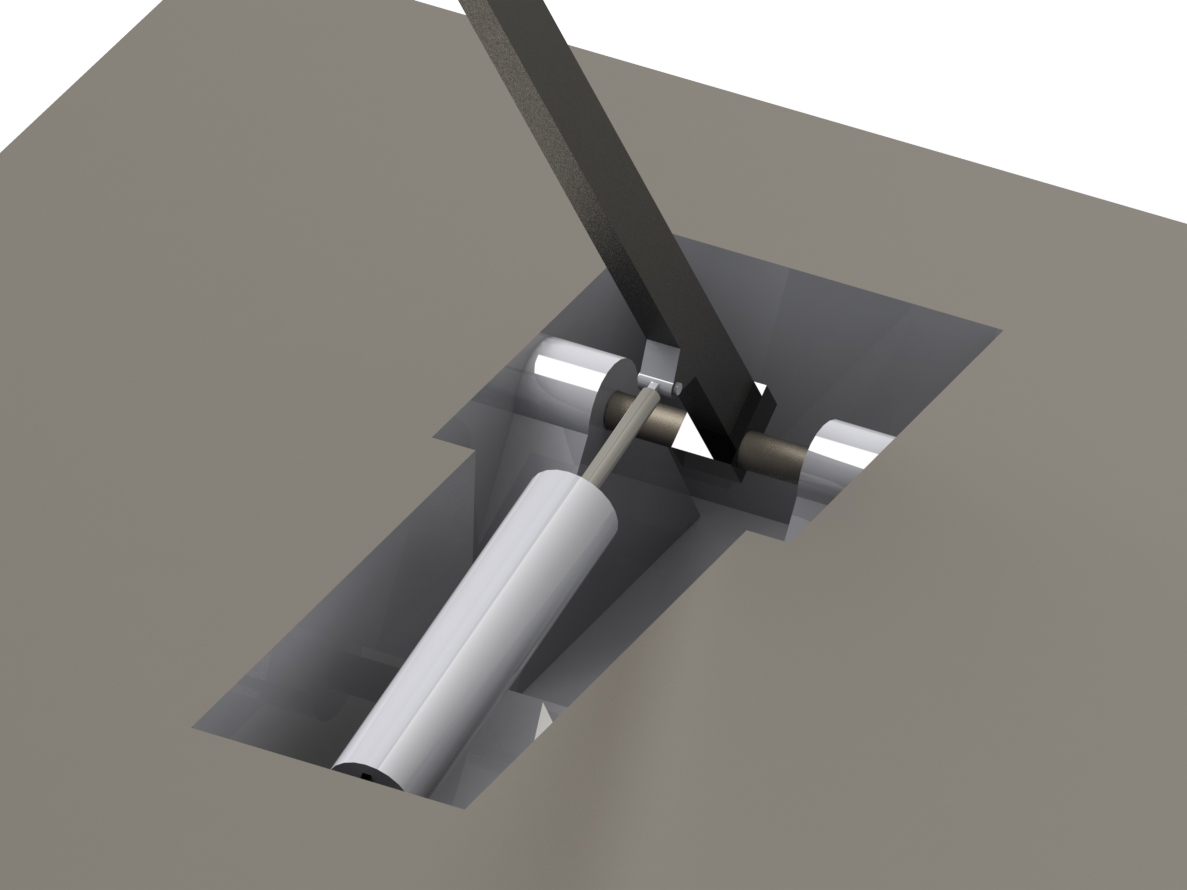
\includegraphics[width=.5\linewidth]{Figures/voice_coil_render.jpg}
    \caption{Boom actuation with a linear voice-coil actuator. By extending and contracting, the linear force is converted to a torque near the base of the boom. This moment in turn controls the angular acceleration of the boom.}
    \label{fig:voice}
\end{figure}
\section{Motion Planner}
\label{sec:wigglesat:planner}
The spacecraft must maintain pointing through a balance of magnetorquer control and boom control. A holistic planning approach is taken due to the following constraints: The magnetorquers cannot be used during payload operations, and the deployable booms must stay within their allowable ranges in position, velocity, and acceleration.  Coarse attitude control has been demonstrated using only magnetorquers \cite{gatherer2019}, but this control strategy is not precise enough for ultra-fine pointing and relies on a varying magnetic field to demonstrate full three-axis actuation. The booms provide full three-degree-of-freedom actuation of the attitude but must avoid violating their actuator constraints. These conditions can be combined into a motion planner that balances magnetorquer use for coarse pointing and momentum desaturation while utilizing the booms for precise pointing during periods of payload operation. Similar to the existing nanosatellite telescopes DeMi \cite{allan2018} and ASTERIA \cite{knapp2020}, this motion planner is tailored to the case where exposures are to be taken during eclipse. This means that the nanosatellite must turn off the magnetorquers for the duration of the $\sim$ 35-minute exposures.  

The angular positions of the booms are described with $\theta \in {\mathbb{R}}^3$, and the angular velocities of the booms as $\dot{\theta} \in {\mathbb{R}}^3$. The control input responsible for boom actuation is the angular acceleration of the booms, denoted as $\alpha \in {\mathbb{R}}^3$.  The dynamics of the booms themselves are modeled as double integrators with angular acceleration as a control input:
\begin{align}
	\ddot{\theta} &= \alpha.
\end{align}
Assuming a zero-order hold on the commanded angular acceleration and discretizing, we have,
\begin{align}
    \begin{bmatrix}\theta_{k+1}\\ \dot{\theta}_{k+1} \end{bmatrix} &= A \begin{bmatrix}\theta_{k} \\ \dot{\theta}_{k} \end{bmatrix}  +  B \alpha_k,
\end{align}
where $A$ and $B$ are a function of the sample time, $dt$:
\begin{align}
    A &= \begin{bmatrix} I_3 & dt\cdot I_3 \\ 0_3 & I_3 \end{bmatrix}, \\ 
    B &= \begin{bmatrix} \frac{1}{2} dt^2 \cdot  I_3 \\ dt \cdot I_3 \end{bmatrix}.
\end{align}
The planning problem is then posed as a convex optimization problem where the optimal sequence of actuator commands, magnetic moment $m$ and boom angular acceleration $\alpha$, are solved for that counter all expected disturbance torques. To ensure that the magnetorquers are never on during payload operations, the optimization formulation conservatively prohibits any magnetorquer usage during periods of eclipse, denoted as indexes $k \in \mathcal{E}$. The full optimization problem can be written as follows: 
\begin{mini}
  {m,\alpha, \theta, \dot{\theta}}{\sum_{k=1}^{N} \|[m_k^T,\,\,\gamma \alpha_k^T,\,\,\beta \theta_k^T,\,\,\sigma \dot{\theta}_k^T]^T\|^2}
  {\label{QP}}
  {}
  \addConstraint{\tau_k=}{ m_k \times b_{\mathbb{B}} -J_{boom}\alpha_k}{\forall k} 
  \addConstraint{\begin{bmatrix}\theta_{k+1}\\ \dot{\theta}_{k+1} \end{bmatrix}=}{ A \begin{bmatrix}\theta_{k} \\ \dot{\theta}_{k} \end{bmatrix}  +  B \alpha_k}{\forall k}
  \addConstraint{m_{min} \leq}{m_k \leq m_{max}}{\forall k}
  \addConstraint{\alpha_{min} \leq}{\alpha_k \leq \alpha_{max}}{\forall k}
  \addConstraint{\theta_{min} \leq}{\theta_k \leq \theta_{max}}{\forall k}
  \addConstraint{\dot{\theta}_{min} \leq}{\dot{\theta}_k \leq \dot{\theta}_{max}}{\forall k}
  \addConstraint{m_k=}{0}{\forall k \in \mathcal{E},}
\end{mini}
where the inertias of the deployable booms are the diagonal entries of $J_{boom}$, the magnetic field of the Earth expressed in the spacecraft body frame is $b_{\mathbb{B}}$, and the disturbance torque is $\tau$. The torque matching constraint and the kinematics of the boom are both enforced as linear equality constraints, and all the state and actuator limits are expressed as box inequality constraints \cite{stellato}. The cost function is a quadratic penalty on control usage for the two sets of actuators, with $\gamma$, $\beta$, and $\sigma$ as tuning parameters. Since the cost function is quadratic and positive definite and the constraints are all linear, problem \ref{QP} can be expressed as a convex Quadratic Program (QP).  There are many readily available and robust QP solvers available that are able to find the global optimum, as well as many specialized solvers for use on embedded systems \cite{mattingley2012,stellato,banjac2017}.  Using one of these tools, a highly performant customized solver can be generated for this specific problem, and can be implemented on compute-constrained flight hardware.
\begin{figure*}
\centering
\includegraphics[width=5in]{Figures/jump_solution.tikz}
\caption{Motion plan for a nanosatellite with control over both boom torques and magnetorquers, given estimated future disturbance torques. During eclipse, when payload operations take place, the nanosatellite is constrained to only use the boom torques due to their precision.}
\label{fig:jumpsolution}
\end{figure*}
\section{Estimation and Control}
\label{sec:wigglesat:control}
Fine-pointing nanosatellites demand the strictest pointing requirements during periods of payload operation. The boom actuators are solely responsible for attitude control during these periods since the magnetorquers are too coarse. The planner is able to leverage predicted disturbance torques to put the booms in a configuration that allows for full controllability during the exposure, but these predicted disturbance torques are not accurate enough to feed forward to the controller during these sensitive payload operations. Instead, during image captures, these disturbance torques will be estimated online in a recursive filter, and the online estimate of the disturbance torque will be incorporated as a feedforward control input. This section details the state estimator and controller combination that is used to maintain high-accuracy pointing during periods of image capture.
\subsection{State Estimator}
The disturbance torques on the nanosatellite are smooth and slowly varying, as shown in Figure \ref{fig:torque}. A Multiplicative Extended Kalman Filter (MEKF) will be used for simultaneous estimation of the attitude, angular velocity, and disturbance torque \cite{markley2014}. Conventional MEKF's on large spacecraft omit the spacecraft's angular velocity from the state due to the accuracy of the onboard gyroscope. Nanosatellites do not have gyroscopes of this caliber and must estimate the angular velocity online as a result. The filter state is denoted $z$, and is augmented to include both the disturbance torque $\hat{\tau}$, as well as its first derivative:
\begin{align}
    z &= \begin{bmatrix} q ^T & \omega^T & \hat \tau^T & \dot{\hat \tau}^T\end{bmatrix}^T,
\end{align}
where $q \in {\mathbb{R}}^4$ is the quaternion describing the rotation from $\mathbb{E}$ to the body frame $\mathbb{B}$, $\omega \in {\mathbb{R}}^3$ is the angular velocity of the nanosatellite, $ \hat \tau \in {\mathbb{R}}^3$ is the disturbance torque, and $\dot{\hat \tau} \in {\mathbb{R}}^3$ is its time derivative. Estimating the disturbance torque derivative allows the filter to better predict and anticipate changes in the disturbance torque. The deterministic dynamics model for the MEKF is as follows:
\begin{align}
\dot{z} &=  \begin{bmatrix} \frac{1}{2} q \otimes (\omega) \\ J^{-1}(\hat \tau  - J_{boom}\alpha - \omega \times J\omega )\\ \dot{ \hat{\tau}} \\ 0
\end{bmatrix}.
\end{align}
These dynamics are discretized using an explicit integrator for a given sample time $\Delta t$, and additive white Gaussian (AWGN) process noise, $\nu_x$, is added as follows:
\begin{align}
    z_{k+1} &= f(z_{k},\alpha_k,\Delta t) + \nu_{x}.
\end{align}
In the measurement model, we assume full measurements of the attitude and angular velocity,
\begin{align}
y &= \begin{bmatrix}q \\ \omega \end{bmatrix} + \nu_y,
\end{align}
where $\nu_y$ is AWGN sensor noise. From here, the MEKF as described in \cite{markley2014} is implemented with the addition of the angular velocity to the estimator state. 

\subsection{Feedback Controller}
By linearizing the dynamics of the nanosatellite about a nominal desired attitude, and replacing the quaternion with an axis-angle vector $\phi\in {\mathbb{R}}^3$, the local error dynamics can be expressed as the following:
% \begin{align}
% \dot{x}_{lqr} = \begin{bmatrix} \dot{\phi} \\ \dot{\omega} \\ \dot{\tau} \\ \ddot{\tau}\end{bmatrix} &= \begin{bmatrix} 0_3 & I_3 & 0_3 & 0_3 \\ 0_3 & 0_3 & J^{-1} & 0_3 \\ 0_3 & 0_3 & 0_3 & I_3 \\ 0_3 & 0_3 & 0_3 & 0_3
% \end{bmatrix}\begin{bmatrix} {\phi} \\ {\omega} \\ {\tau} \\ \dot{\tau}\end{bmatrix} + \begin{bmatrix}0_3 \\ -J_{boom} \\ 0_3 \\ 0_3 \end{bmatrix} \alpha 
% \end{align}
\begin{align}
\dot{x}_{lqr} = \begin{bmatrix} \dot{\phi} \\ \dot{\omega}\end{bmatrix} &= \begin{bmatrix} 0 & I  \\ 0 & 0 
\end{bmatrix}\begin{bmatrix} {\phi} \\ {\omega} \end{bmatrix} + \begin{bmatrix}0 \\ -J_{boom} \end{bmatrix} \alpha .
\end{align}
From here, the dynamics can be discretized assuming a zero-order hold on $\alpha$, and a feedback gain $K$ is solved for that minimizes the following infinite-horizon Linear Quadratic Regulator (LQR) cost function:
\begin{align}
\ell(x,u) = \frac{1}{2}\sum_{k=0}^\infty x_{k}^TQx_{k} + \alpha_k^TR\alpha_k , 
\end{align}
where $Q\in {\mathbb{R}}^{6 \times 6}$ and $R\in {\mathbb{R}}^{3\times 3}$ are positive definite diagonal matrices \cite{stengel1994}. The resulting control law takes the form,
\begin{align}
    u = -Kx_{lqr} - J_{boom}^{-1}\hat{\tau},
\end{align}
where $\hat{\tau}$ is the estimated disturbance torque from the MEKF.
\begin{figure}
    \centering
    \includegraphics[width=.4\linewidth]{Figures/control/torque.tikz}
    \caption{Disturbance torques over a 45 minute period. These torques are smooth and slowly varying, making estimation of this torque possible in a Kalman Filter.}
    \label{fig:torque}
\end{figure}
% \begin{figure*}
% \centering
% \includegraphics[width=5in]{Figures/jump_solution.tikz}
% \caption{Motion plan for a nanosatellite with control over both boom torques and magnetorquers, given estimated future disturbance torques. During eclipse, when payload operations take place, the nanosatellite is constrained to only use the boom torques due to their precision.}
% \label{fig:jumpsolution}
% \end{figure*}
\section{Numerical Experiments}
\label{sec:wigglesat:experiments}
\begin{figure}
    \centering
    \includegraphics[width=.5\linewidth]{Figures/control/mekf_converge.tikz}
    \caption{MEKF estimation errors for the unknown disturbance torque, as well as 3-$\sigma$ bounds from the covariance. By modeling the disturbance torques as a double integrator system, where both the torque and its time derivative are estimated, the MEKF is able to converge on accurate estimates of the true torque values in less than 1 minute.}
    \label{fig:mekf}
\end{figure}
\begin{figure}
    \centering
    \includegraphics[width=.5\linewidth]{Figures/control/loop.tikz}
    \caption{Closed-loop yaw and pitch error with an attitude sensor standard deviation of 1 arcsecond. The combined estimator and controller are able to maintain sub-arcsecond pointing even in the presence of the sensor noise and unknown disturbance torques.}
    \label{fig:loop}
\end{figure}
\begin{figure}
    \centering
    \includegraphics[width=.5\linewidth]{Figures/control/mc.tikz}
    \caption{For each attitude sensing error, a series of simulations were run to estimate the mean and 3-$\sigma$ bounds for the RMS body pointing error. Despite all the simulations using the same gyroscope, the estimator and controller combination is able to continue driving down the body pointing error with the sensing error.}
    \label{fig:mc}
\end{figure}

All experiments were run in Julia \cite{bezanson2017}, using the optimization modeling language JuMP \cite{lubin2015} with Mosek \cite{mosekaps2014} as the solver for the motion-planning problem.  All of the code used for the experiments is readily available at \url{https://github.com/RoboticExplorationLab/WiggleSat.jl}.

To test the planning and control algorithms presented in this paper, a nanosatellite in a low-Earth orbit with an altitude of 420 km, inclination of $51.4^\circ$, and eccentricity of $0.00108$ is considered. The orbit is propagated with accelerations from a high-order gravity model, atmospheric drag, solar radiation pressure, and third body contributions from the Moon and the Sun \cite{montenbruck2002}. The disturbance torques as described in Section \ref{sec:wigglesat:simenv} are then calculated given the desired attitude.  The attitude measurement has a standard deviation of 1 arcsecond \cite{douglas2021}, the gyroscope is modeled after the Honeywell GG1320AN with an angle random walk of 0.0035 deg/$\sqrt{hr}$, and the sample rate on the sensors, filter, and controller is 1 Hz \cite{honeywell}.

The motion planner, as detailed in Section \ref{sec:wigglesat:planner}, is used to calculate a nominal control plan for both the magnetorquers and the booms. With a time horizon of 4 hours, the planner is able to account for two eclipse periods where the magnetorquers are unavailable. The solution from the planner is shown in Figure \ref{fig:jumpsolution}, with the nominal control plans for both boom torques as well as commanded magnetic moment. The planner effectively balances momentum management with the requirement to put the arms in a configuration prior to eclipse that allows for full controllability throughout the duration of the eclipse.

During eclipse, the estimator and controller designed in Section \ref{sec:wigglesat:control} are used to maintain the desired attitude.   Instead of relying on the predicted disturbance torque, an MEKF is used to estimate both the attitude and angular velocity, as well as the disturbance torque and its time derivative. The convergence of this filter on the unknown disturbance torque is shown in Figure \ref{fig:mekf}. Even with a poor initialization of all zeros for the estimate of the disturbance torque, the filter is able to converge on the true value within one minute of operation.

The pointing performance of the combined estimator and controller is shown in Figure \ref{fig:loop}. Here, the initial condition starts outside the 1-arcsecond error circle, and the controller is able to keep the error inside the circle for a Root Mean Square (RMS) body pointing error of 0.39 arcseconds. To better evaluate the robustness and performance of this estimator and controller combination, this same simulation was run for a variety of initial conditions with a range of attitude sensing errors. The RMS body pointing error as a function of this attitude sensing error is shown in Figure \ref{fig:mc}, where the mean body pointing performance as well as three-sigma bounds are shown. We also note that the filter performs well enough that body-pointing errors are able to decrease with attitude sensing error, despite using the same gyroscope for all simulations. 
\section{Conclusions}
\label{sec:wigglesat:conclusion}
This paper proposes a novel attitude actuation strategy for fine-pointing nanosatellites. The new approach abandons traditional high-frequency reaction wheels in favor of low-frequency actuated booms. As shown by a spectral analysis of the environmental disturbance torques, these low-frequency deployable booms are a much better fit for the slowly varying disturbance torques encountered in low-Earth orbit. By performing control in the same frequency range as these disturbances, many of the complications that reaction wheels introduce, including high-frequency jitter and excitement of flexible structural modes, can be avoided. This actuation methodology results in finer body-pointing performance, reducing the need for second-stage correction systems to point sensitive payloads.

Control of a spacecraft equipped with the proposed boom actuators was demonstrated via a convex-optimization-based motion planner paired with an MEKF estimator and LQR controller during sensitive payload operations. This planner was able to balance magnetorquer usage and boom actuation to combat environmental disturbances, reason about actuator limits and boom constraints, and avoid magnetorquer usage during periods of eclipse for improved payload operations. This optimization problem was formulated as a quadratic program and can be solved quickly and reliably onboard spacecraft with limited computing resources. 




%%% Local Variables:
%%% coding: utf-8
%%% mode: latex
%%% TeX-engine: xetex
%%% TeX-master: "../thesis"
%%% End: